\newpage
\section{Overview}
\label{chapter1}
The SafeSU (Safe Statistics Unit) is an AHB slave capable of monitoring SoC events, enforce contention control, and identifying profiling errors on run-time.
Figure "\ref{fig:blkdia}" shows the structure of the unit. It is composed of an ahb wrapper (\textit{ahb\_wrapper.vhd}) that maps the SystemVerilog implementation into a VHDL module that can be instanced in SELENE and De-RISC SoCs.  The SystemVerilog AHB interface (\textit{pmu\_ahb.sv}) offers support for a subset of AHB requests. This module also instances the interface agnostic SafeSU (\textit{PMU\_raw.sv}). The latter is used as the generator of the statistic unit. It generates the memory map and the instances for each of the features.\\
\\
The main features are:\\
\begin{itemize}
	\item \textbf{Self-test:} Allows to configure the counters' inputs to a fixed value bypassing the crossbar and ignoring the inputs. This mode allows for tests of the software and the unit under known conditions.
	\item \textbf{Crossbar:} Allows to route any input event to any counter.
	\item \textbf{Counters:} Group of simple counters with settable initial values and general control register.
	\item \textbf{Overflow:} Detection of overflow for counters, interrupt capable with dedicated interruption vector and per counter interrupt enable.
	\item \textbf{Quota:} Deprecated \textit{(It may be excluded in a future release)}
	\item \textbf{MCCU }(Maximum Contention Control Unit) : Contention control measures for each core. Interruption capable after a threshold of contention is exceeded. It accepts real contention signals or estimation through weights.
	\item \textbf{RDC }(Request Duration Counters): Provides measures of the pulse length of a given input signal (watermark). It can be used to determine maximum latency and cycles of uninterrupted contentions. Each of the counters can trigger an interrupt at a user-defined threshold.
\end{itemize}

The default configuration of this unit supports 4 cores and 32 input signals. In future releases such parameters (VHDL generics) will be exposed to the top level.
\begin{figure}[H]
	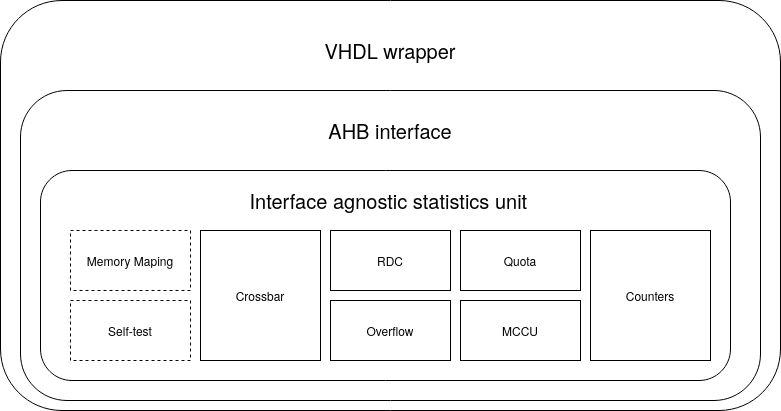
\includegraphics[keepaspectratio,width=\columnwidth]{img/GRLIB_SU.png}
	\caption{Block diagram statistics unit structure}
	\label{fig:blkdia}
\end{figure}
